\chapter{Introduction}
\label{chap:intro}
Probabilities describe degrees of belief, and probabilistic inference describes rational reasoning under uncertainty. Undoubtedly, probabilistic models have exploded onto all the sciences of inference under uncertainty: machine learning, information retrieval, applied statistics and artificial intelligence. However, it's not easy for common programmers to describe the probabilistic models and encode the probabilistic inference process. Especially when the probabilistic models become complicated, the complexity to describe them and to perform inference will be raised subsequently. Just as programming beyond the simplest algorithms requires tools for abstraction and composition, complex probabilistic modeling requires new progress in model representation - probabilistic programming languages. Probabilistic programming languages are in the spotlight, which provide compositional means for describing complex probability distributions and performing efficient probabilistic inference. ~\cite{goodman}.

The goal of probabilistic programming is to enable probabilistic modeling and machine learning to be accessible to the working programmer, who has sufficient domain expertise, but perhaps not enough expertise in probability theory or machine learning. We wish to hide the details of inference inside the compiler and runtime, and enable the programmers to express models using their domain expertise and dramatically increase the number of programmers who can benefit from probabilistic modeling. In probabilistic programming, modeling and inference have been disentangled.

In this chapter, the background information of probabilistic programming will be introduced. In section ~\ref{sec:pp}, we will illustrate what is probabilistic programs and will give some simple examples. In section ~\ref{sec:pgm}, we will introduce probabilistic graphical models, especially the relationships between probabilistic programs and other probabilistic models that readers may have encountered before. Two kinds of probabilistic graphical models will be discussed: Bayesian networks and Markov networks. In section ~\ref{sec:inferintro}, we will elaborate on the probabilistic inference technologies and show some examples of probabilistic inference problems. In section ~\ref{sec:language}, the formalized probabilistic programming language will be defined and the difference between common programming languages and probabilistic programming languages according to syntax and semantics will be illustrated. 

\section{Probabilistic Programs}
\label{sec:pp}
\textit{Probabilistic programs} are ``usual" programs (written in languages like C, Java, Ocaml or Lisp) with two additional constructs: (1) the ability to draw values at random from distributions (like gaussian, gamma, etc.), and (2) the ability to condition values of variables in a program via observe statements (which can incorporate data from real world observations into a probabilistic program). ~\cite{gordon2014}. A variety of probabilistic programming languages and systems have been proposed, including BUGS ~\cite{bugs}, Church ~\cite{church}, FACTORIE ~\cite{factorie}, Infer.NET ~\cite{infernet}, Dimple ~\cite{dimple}, etc. However, unlike usual programs which are written for the purpose of being executed, the purpose of a probabilistic program is to implicitly specify a probability distribution. 

We introduce the syntax and semantics of probabilistic programs using two simple probabilistic programs from Figure ~\ref{fig:pp_simple_eg}. This is an example written in \textbf{Probabilistic C}. Drawing from a Bernoulli distribution with mean 0.5 can be seen as tossing fair coins. The program in the top, Example $1(a)$, tosses two fair coins, and respectively assigns the outcomes of these coin tosses to the Boolean variables $c_1$ and $c_2$, and returns $(c_1, c_2)$. The semantics of this program is the expectation of its return value. In this case, the return value will be $(1/2, 1/2)$. Since we have that 
\begin{align*}
  P & ( c_1 = false, c_2 = false) =\\
  P & (c_1=false, c_2=true) = \\
  P & (c_1=true, c_2=false) = \\
  P & (c_1=true, c_2=true) = 1/4
\end{align*}
we have that the expectation on the return value is given by 
\begin{align*}
  1/4 \times (0, 0) + 1/4 \times (0, 1) + 1/4 \times (1, 0) + 1/4 \times (1, 1) = (1/2, 1/2)
\end{align*}
where we treated true as $1$ and false as $0$.

The program in Example $1(b)$ is slightly different from Example $1(a)$. It has an observe statement $observe(c_1 \| c_2)$ before returning the value of $(c_1,c_2)$. The observe statement blocks runs which do not satisfy the boolean expression $c_1 \| c_2$ and does not permit those executions to happen. Executions that satisfy $c_1 \| c_2$ are permitted to happen. It is sort of a condition that the varibales need to meet. Thus the semantics of the program is the expected return value conditioned by $(c_1 \| c_2)$, the permitted executions. Since conditioning by permitted executions yields
\begin{align*}
  P & (c_1=false,c_2=false) = 0 \\
  P & (c1=false,c2=true) = \\
  P & (c1=true,c2=false) = \\
  P & (c1=true,c2=true) = 1/3
\end{align*}
we have that the different expected return value which is 
\begin{align*}
  0 \times (0,0) + 1/3 \times (0,1) + 1/3 \times (1,0) + 1/3 \times (1,1) = (2/3,2/3).
\end{align*}

\begin{figure}
    \centering
    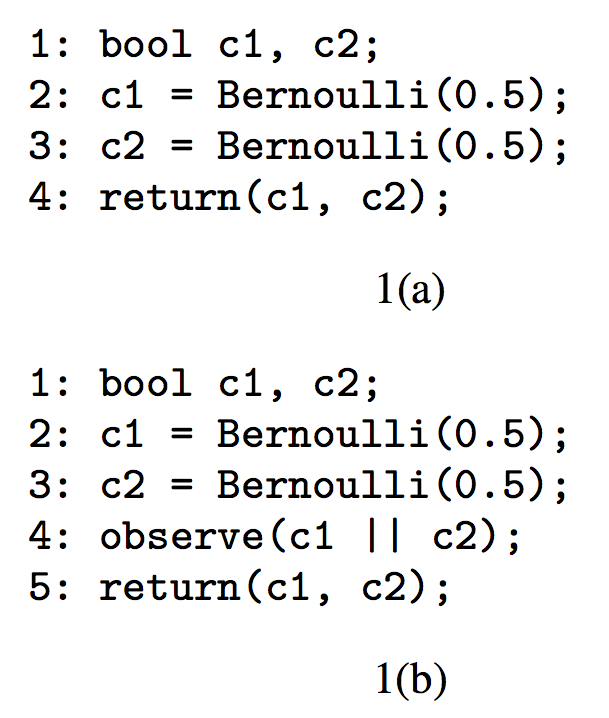
\includegraphics[width=0.4\textwidth]{figures/pp_simple_eg.png}
    \caption{Simple probabilistic programs}
    \label{fig:pp_simple_eg}
\end{figure}

Another example of the probabilistic programs is for Latent Dirichlet Allocation (LDA), which can be seen in Figure ~\ref{fig:lda}. In the LDA example, the words in blue represent probability distributions with the arguments as parameters of the distributions. Each time a value can be sampled from the specified probability distributions, such as \textbf{dirichlet}, \textbf{multinomial}, \textbf{gaussian}, etc. The trace of the sampled value meet the requirement of the corresponding probability distribution. Compared with the LDA program coding in some comman languages like C, Python, or Matlab in hundreds of lines, which contains both of the modeling code and inference code, programming in probabilistic programming language is a big relief for programmers and is much easier for the programmers to read the program.

\begin{figure}
    \centering
    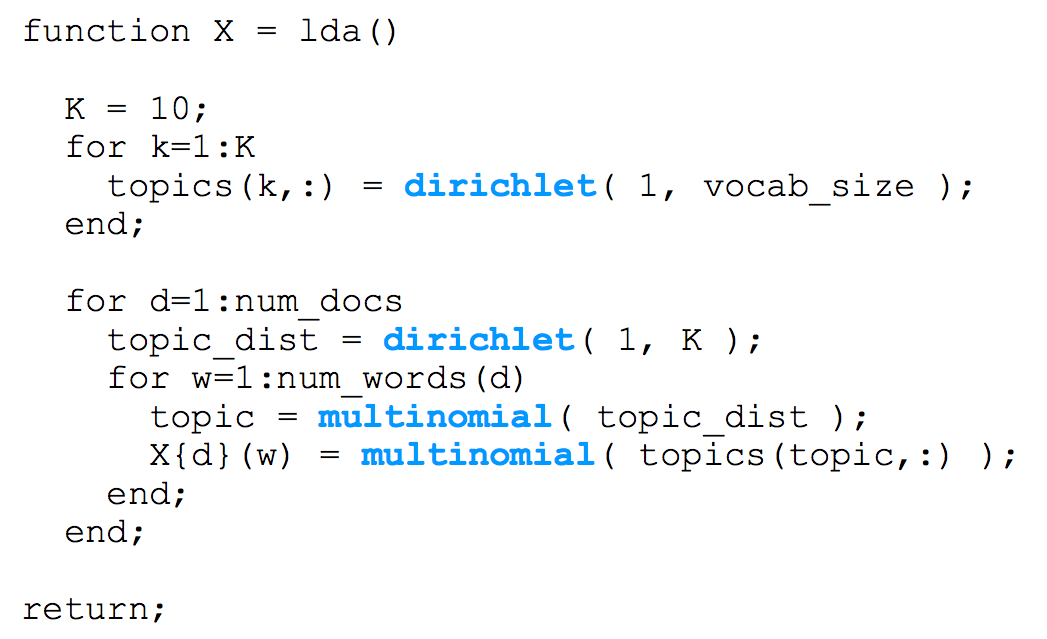
\includegraphics[width=0.8\textwidth]{figures/lda_eg.png}
    \caption{Probabilistic program example: LDA.}
    \label{fig:lda}
\end{figure}


\section{Probabilistic Graphical Model}
\label{sec:pgm}
Probabilistic programs can be used to represent probabilistic graphical models ~\cite{pgm}, which use graphs to denote conditional dependences between random variables.

\begin{figure}
    \centering
    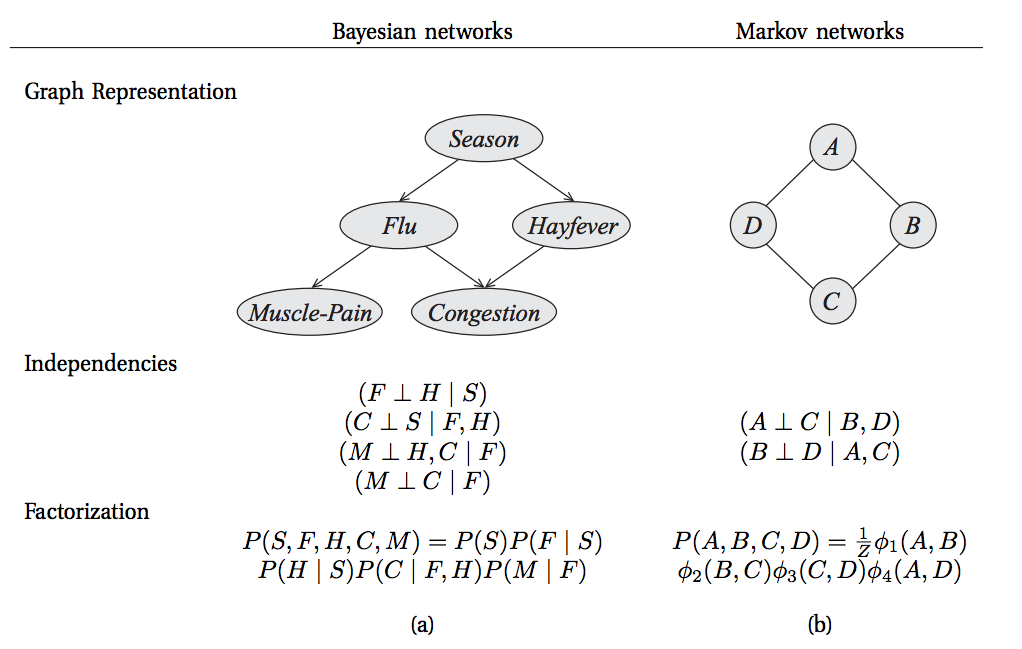
\includegraphics[width=\textwidth]{figures/pgm.png}
    \caption{Probabilistic graphical models in different perspectives: the graphical representation (top); the independencies induced by the graph structure (middle); the factorization induced by the graph structure (bottom). (a) A sample Bayesian network. (b) A sample Markov network.}
    \label{fig:pgm}
\end{figure}

\textit{Probabilistic graphical models(PGM)} use a graph based representation as the basis for compactly encoding a complex distribution over a high-dimensional space. In the graphical representation illustrated in Figure ~\ref{fig:pgm}, the nodes correspond to the variables in the domain, and the edges correspond to direct probabilistic interactions between them. For example, in Figure ~\ref{fig:pgm}, the top of (a) illustrates one possible graph structure for a patient example, where \texttt{Flu} depends on \texttt{Season} and \texttt{Congestion} depends on \texttt{Hayfever}. In this graph, we can see that there is no direct edge between \texttt{Muscle Pain} and \texttt{Season}, but both interact directly with \texttt{Flu}. There are two perspectives that one can use to interpret the structure of this graph. From one perspective, the graph is a compact representation of a set of independencies that hold in the distribution; these properties take the form $X$ is independent of $Y$ given $Z$, denoted $(X \bot Y | Z)$, for some subsets of variables $X, Y ,Z$. In this example, the distribution satisfies the conditional independence $(Congestion \bot Season | Flu, Hayfever)$. This statement asserts that
\begin{align*}
P(Congestion | Flu, Hayfever, Season) = P(Congestion | Flu, Hayfever);
\end{align*}
that is, if we are interested in the distribution over the patient having congestion, and we know whether he has the flu and whether he has hayfever, the season is no longer informative. But this assertion does not imply that \texttt{Season} is independent of \texttt{Congestion}. Figure ~\ref{fig:pgm}a (middle) shows the set of independence assumptions associated with the graph in Figure ~\ref{fig:pgm}a (top).

The other perspective is that the graph model describes a skeleton for compactly representing a high dimensional factor graph. Rather than encoding the probability of every possible assignment to factor all of the variables in our domain, we can ``break up" the distribution into smaller factors, each over a much smaller space of possibilities. We can then define the overall joint distribution as a product of these factors. For example, Figure ~\ref{fig:pgm}a (bottom) shows the factorization of the distribution associated with the graph in Figure ~\ref{fig:pgm}a (top). It asserts, for example, that the probability of the event “spring, no flu, hayfever, sinus congestion, muscle pain” can be obtained by multiplying five numbers:
\begin{align*}
  P&(Season = spring)\\
  P&(Flu = false | Season = spring)\\
  P&(Hayfever = true | Season = spring)\\
  P&(Congestion = true | Hayfever = true,Flu = false)\\
  P&(Muscle Pain = true | Flu = false)
\end{align*}
The graph structure defines the factorization of a distribution $P$ associated with it - the set of factors and the variables that they encompass.

We will describe two families of graphical representations of distributions. One, called Bayesian networks, uses a directed graph, as shown in Figure ~\ref{fig:pgm}a (top). The second, called Markov networks, uses an undirected graph, as illustrated in Figure ~\ref{fig:pgm}b (top). It can be viewed as defining a set of independence assertions (Figure ~\ref{fig:pgm}b (middle) or as encoding a compact factorization of the distribution as showed in Figure ~\ref{fig:pgm}b (bottom). Both representations provide the duality of independencies and factorization, but they differ in the set of independencies they can encode and in the factorization of the distribution that they induce. In this paper we will focus more on Bayesian networks.


\subsection{Bayesian Networks}
A Bayesian network structure is a directed, acyclic graph $G$, where each vertex $s$ of $G$ is interpreted as a random variable $X_s$ (with unspecified distribution) ~\cite{heckerman}.
A Bayesian network $(G, P)$ consists of
\begin{itemize}
  \item a BN structure G and
  \item a set of conditional probability distributions (CPDs) $P(X_s | Pa_{X_s})$, where $Pa_{X_s}$ are the parents of node $X_s$ such that 
  \item $(G, P)$ defines a joint distribution
  \begin{align*}
    P(X_i, \dots, X_n) = \prod_i P(X_i | Pa_{X_i})
  \end{align*}
\end{itemize}
For Bayesian networks, there are two kinds of different inference problems.~\cite{heckerman1998tutorial}.

\subsubsection{Learning Probabilities in a Bayesian Network}
Bayesian networks can be used to answer probabilistic queries given the prior probabilities and conditional probabilities. For instance, in a Bayesian network there are two random variable $X, Y$ where $X$ is observed and $Y$ is unobserved. And we know that the dependency probability of $P(Y | X)$, then we can learn the joint probability of $X, Y$ where 
\begin{align*}
  P(X, Y) = P(X) \times P(Y | X).
\end{align*}
The process of computing the posterior distribution of variables given evidence is called \textit{probabilistic inference}. More details can be seen in Section \ref{sec:inferintro}. On the other hand, we can choose a value for a random variable in its domain to maximize a likelihood probability or minimize a cost function in a Bayesian network. 

\subsubsection{Learning parameters and structures}
Sometimes the given Bayesian network has some unobserved variables without knowing the exact distributions that the variables follow. Then we can estimate the parameters of the distribution based on the probability of observed variables and the structure of the graph. We can also estimate the parameter from data, for example, using the maximum likelihood approach. There are also some other appoaches to this problem like the expectation maximization(EM) algorithm and the Viterbi algorithm for Hidden Markov Model(HMM). There are also some sampling algorithms that to learn the parameters by viewing the parameters as additional hidden variables.

For structure learning, when defining the probabilistic graphical model is pretty complex for humans or there are many probabilistic models one can choose from, we can learn the network structure from data. Doing structure learning automatically is still a challenge. 

\subsection{Markov Networks}
\textit{Markov network}, or \textit{Markov random field} is a set of random variables having a Markov property described by an undirected graph. A Markov random field is similar to a Bayesian network in its representation of dependencies. The differences being that Bayesian networks are directed and acyclic, whereas Markov networks are undirected and may be cyclic. Thus, a Markov network can represent certain dependencies that a Bayesian network cannot (such as cyclic dependencies). On the other hand, it can't represent certain dependencies that a Bayesian network can (such as induced dependencies).~\cite{markov}.\\

In our framework, the language targets to describe Bayesian networks and solves the query of inferring unobserved variables by probabilistic inference.

\section{Probabilistic Inference}
\label{sec:inferintro}
\textit{Probabilistic inference} is the problem of computing an explicit representation of the probability distribution implicitly specified by a probabilistic program. If the probability distribution is over a large number of variables, an explicit representation of the joint probability distribution may be both difficult to obtain efficiently, and unnecessary in the context of specific application contexts. The desired output of inference may vary from different applications. For example, we may want to compute the expected value of some function $f$ with respect to the distribution (which may be more efficient to calculate without representing the entire joint distribution). Alternatively, we may want to calculate the most likely value of the variables, which is the mode of the distribution. Or we may want to simply draw a set of samples from the distribution, to test some other system which expects inputs to follow the modeled distribution. ~\cite{gordon2014}.

\begin{figure}
    \centering
    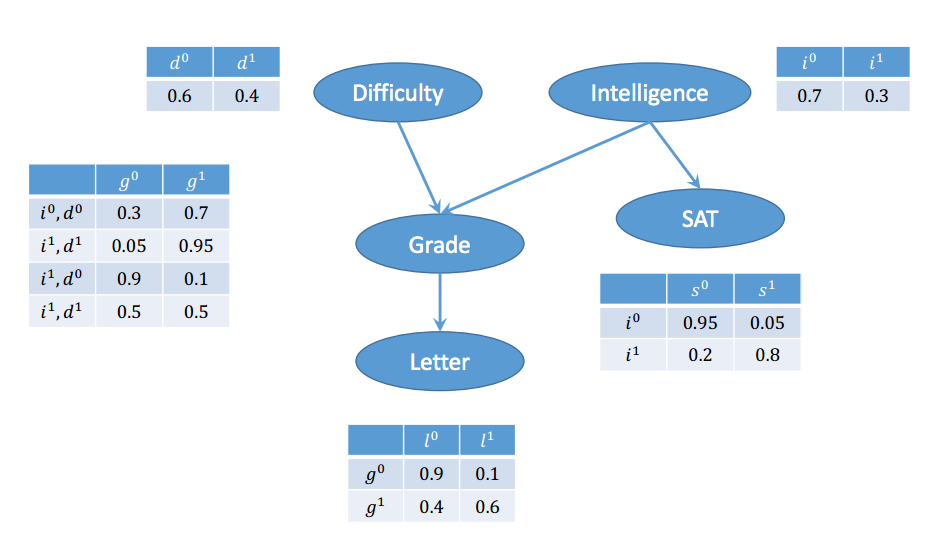
\includegraphics[width=0.9\textwidth]{figures/inference.png}
    \caption{A student example to show probabilistic inference.}
    \label{fig:infer_eg}
\end{figure}

Figure ~\ref{fig:infer_eg}. gives an example of inference problem. The variable \textit{Difficulty} describes the difficulty of the courses with probability $0.6$ to be not hard, namely $d_0$, and with probability $0.4$ to be hard, that is $d_1$. Other variables share the similar meaning with \textit{Difficulty}. If we want to know the probability of the student getting $Letter = l_1$ under the condition that his grade $Grade = g_1$, then this is an inference problem with the formal representation $P (L = l_1 | G = g_1)$. Also, if we want to know the probability of the student getting $Grade = g_1$ under he/she has already get the $Letter = l_1$, which is a backward process compared with the previous conditional probability, this is also the problem of probabilistic inference with the formal representation $P (G = g_1 | L = l_1)$.

Threre are two kinds of inference technologies, exact inference and approximate inference. The exact inference methods include elimination algorithm, namely sum-product algorithm, which computes the probability by summing the joint probability thus to eliminate the non-observed and non-query variables; message-passing algorithm, which is an improvement of elimination algorithm if we want to caculate more than one marginal probability. In message-passing algorithm, the intermediate terms of probability will be viewd as ``messages'' and the inference process will be considered as local computation and routing of messages. All of the exact inference algorithms have the complexity that is exponential to the size of the graph. The approximate inference algorithms include stochastic Markov chain Monte Carlo(MCMC) simulation ~\cite{mcmc} which contains many sampling algorithms like Gibbs sampling, Metropolis-Hastings Algorithms and importance sampling, mini-bucket elimination, generalized belief propagation, and variational methods.

\subsection{Markov Chain Monte Carlo}
In this paper, we focused on the MCMC simulation methods to do inference. MCMC techniques are often applied to solve integration and optimisation problems in large dimensional spaces. In Bayesian inference and learning, given some unknown variables $x \in \mathscr{X}$ and data $y \in \mathscr{Y}$. the following typically intractable integration problems are central to Bayesian statistics. 
\begin{itemize}
  \item Normalization. To obtain the posterior $p(x | y)$ given the prior $p(x)$ and likelihood $p(y | x)$, the normalising factor in Bayes' theorem needs to be computed
    \begin{align*}
      p(x | y) = \frac{p(y | x)p(x)}{\int_{\mathscr{X}} p(y | x')p(x')dx'}
    \end{align*}
  \item Marginalisation. Given the joint posterior of $(x, z) \in \mathscr{X} \times \mathscr{Z}$, we may often be interested in the marginal posterior
    \begin{align*}
      p(x | y) = \int_{\mathscr{Z}} p(x, z| y)dz.
    \end{align*}
  \item Expectation. The objective of the analysis is often to obtain summary statistics of the form 
    \begin{align*}
      \mathbb{E}_{p(x|y)}(f(x)) = \int_{\mathscr{X}}f(x)p(x | y)dx
    \end{align*}
\end{itemize}
for some function of interest $f : \mathscr{X} \rightarrow \mathbb{R}^{n_f}$ integrable with respect to $p(x | y)$. Examples of appropriate functions include the conditional mean, in which case $f(x) = x$, or the conditional covariance of $x$ where $f(x) = xx' - \mathbb{E}_{p(x|y)}(x)\mathbb{E}'_{p(x|y)}(x)$.

The idea of Monte Carlo simulation is to draw an i.i.d. set of samples $\{x^{(i)}\}_{i = 1}^N$ from a target density $p(x)$ defined on a high-dimensional space $\mathscr{X}$. These $N$ samples can be used to approximate the target density with the following empirical point-mass function
\begin{align*}
  p_N(x) = \frac{1}{N} \sum_{i = 1}^N \sigma_{x^{(i)}}(x)
\end{align*}
where $\sigma_{x^{(i)}}(x)$ denotes the delta-Dirac mass located at $x^{(i)}$.

\begin{figure}
    \centering
    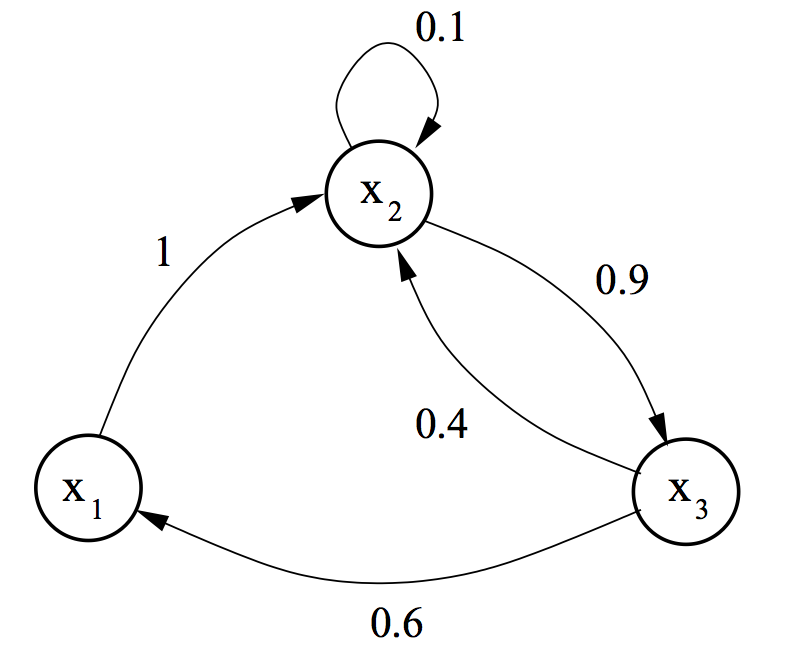
\includegraphics[width=0.7\textwidth]{figures/mcmc.png}
    \caption{Transition graph for a Markov chain example}
    \label{fig:mcmc}
\end{figure}

MCMC is a strategy for generating samples $x^{(i)}$ while exploring the state space $\mathscr{X}$ using a Markov chain mechanism. To introduce Markov chains on finite state spaces, suppose that $x^{(i)}$ can only take $s$ discrete values $x^{(i)} \in \mathscr{X} = { x_1, x_2, \dots, x_s}$. The stochastic process $x^{(i)}$ is called a Markov chain if
\begin{align*}
  p(x^{(i)} | x^{(i - 1), \dots, x^{(1)}}) = T(x^{(i)} | x^{(i - 1)})
\end{align*}
where $T$ is a transition function. That is, the evolution of the chain in a space $\mathscr{X}$ depends solely on the current state of the chain and fixed transition matrix. Figure ~\ref{fig:mcmc} gives an example of transition graph for Markov chain with $\mathscr{X} = \{x_1, x_2, x_3\}$.
 
We leveraged two methods of MCMC technologies for approximate inference including rejection sampling ~\cite{reject} and Metroplis-Hastings algorithm ~\cite{mh}. More details can be found in Chapter \ref{chap:approach}.

\section{Probabilistic Programming Language}
\label{sec:language}
\textit{Probabilistic Programming Language(PPL)} extends a well-specified deterministic programming language with primitive constructs for random choice. Just as with deterministic programming languages, there are probabilistic languages in the imperative, functional, and logical paradigms. We will take one of the probabilistic programming language \textbf{Probabilistic C} ~\cite{probc} as example, which is a C-like imperative programming language with two additional statements:
\begin{enumerate}
  \item The probabilistic assignment $``x \sim Dist(\bar{\theta})"$ draws a sample from a distribution $Dist$ with a vector of parameters $\bar{\theta}$, and assigns it to the variable $x$. For instance, the statement $``x \sim Gaussian(\mu, \sigma)"$ draws a value from a $Gaussian$ distribution with mean $\mu$ and standard deviation $\sigma$, and assigns it to the variable $x$.
  \item The observe statement $``observe(\varphi)"$ conditions a distribution with respect to a predicate or condition $\varphi$ that is defined over the variables in the program. In particular, every valid execution of the program must satisfy all conditions in observe statements that occur along the execution.
\end{enumerate}

\begin{figure}
    \centering
    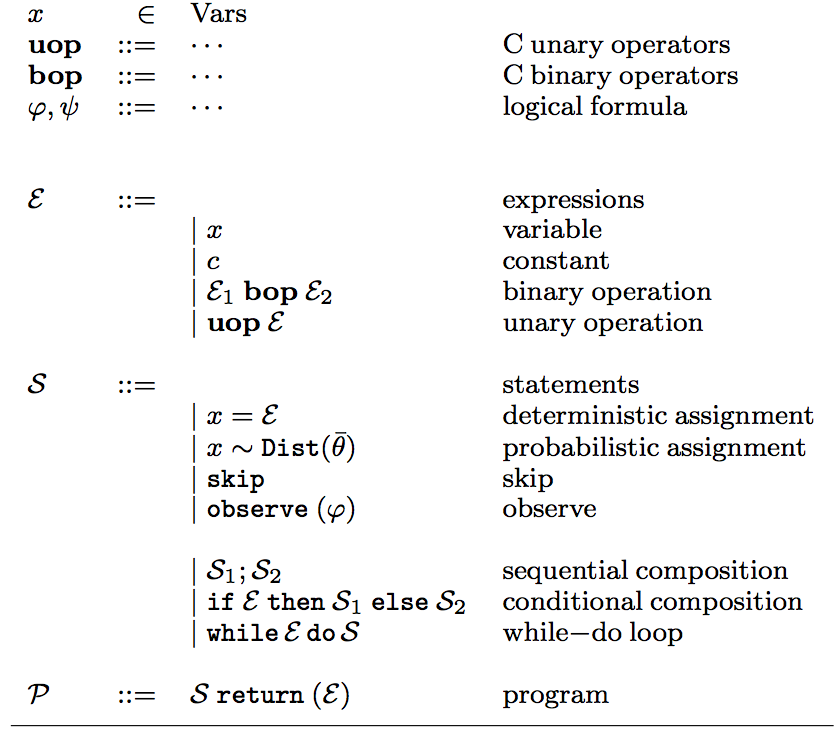
\includegraphics[width=0.6\textwidth]{figures/prob_syntax.png}
    \caption{Syntax of PROB}
    \label{fig:prob_syntax}
\end{figure}

The syntax of \textbf{Probabilistic C} is formally described in Figure ~\ref{fig:prob_syntax}. A program consists of a statement and a return expression. Variables have base types such as int, bool, float and double. Expressions include variables, constants, binary and unary operations.

Statements include primitive statements (deterministic assignment, probabilistic assignment, observe, skip ) and composite statements (sequential composition, conditionals and loops). \\

In summary, probabilistic graphical models are the representations of the structure of probability distributions. One can derive the explicit representation of probability distribution by performing probabilistic inference. Probabilistic programming language can describe probabilistic graphical models and query some conditional probability or joint probability. So probabilistic programs have two extra feature than usual programs: 
\begin{enumerate}
  \item Draw samples from probability distribution
  \item Query some probability automatically.
\end{enumerate}

In Chapter ~\ref{chap:related}, the related work will be introduced including the state of the art probabilistic programming languages and systems. In Chapter ~\ref{chap:approach}, we will elaborate on the approach of the design of the portable probabilistic programming framework. More specifically, an overview of our framwork will be showed in Section ~\ref{sec:overview}. The syntax of the declarative language is illustrated in Section ~\ref{sec:syntax} and the implementation of the probabilistic library is showed in Section ~\ref{sec:distr}. The algorithms of probabilistic inference are elaborated in Section ~\ref{sec:infer}. And the principles and usage of the APIs for other common programming languages is illustrated in Section ~\ref{sec:api}. In Chapter ~\ref{chap:eval}, the implementations of our framework and the case studies of the performance of the framework will be showed. In Chapter ~\ref{chap:conclusion}, we will conclude our work and the future work that can be done based on our framework. 

